\documentclass[12pt,twoside,a4paper]{report}

%---------------------------------------------------------------------
% define packages
\usepackage{graphicx}
\DeclareGraphicsExtensions{.jpg, .png , .pdf}
\usepackage[margin=2cm]{geometry}
\usepackage{color}
\usepackage{longtable}
\definecolor{grey}{rgb}{0.5,0.5,0.5}

%---------------------------------------------------------------------
% define some commands
\newcommand{\tl}{\textless}
\newcommand{\tg}{\textgreater}
\newcommand{\tbf}{\textbf}
\newcommand{\tit}{\textit}
\newcommand{\hs}{\hspace{1mm}}
\renewcommand\thesection{\arabic{section}}

\setlength{\parindent}{0cm}

%---

\title{Technical Testsuite v2.2\\User Guide}
%---------------------------------------------------------------------

\begin{document}

\maketitle
\setcounter{tocdepth}{1}
\tableofcontents 

%---------------------------------------------------------------------
\section{Introduction}

The main goal of the testsuite is to check technical correctness of a COSMO model version (see section Section 6.5 of the COSMO coding standards). The testsuite is implemented using the Python programming language.
Based on a set of given model configurations (which can be defined by the user, for example COSMO-RU, COSMO-EU or COSMO-2), the test suite creates modifications of this configuration and launches a short simulation for each of the new configurations. The software then verifies that:
\begin{itemize}
\item the simulations run without aborting or crashing
\item the results are within rounding error with respect to a reference simulation
\item the code gives bit identical results with different processor configurations or I/O configurations
\item restart functionality is working and gives bit identical results
\end{itemize}

Additional user defined verifications (so called "checkers") can be specified.

%---------------------------------------------------------------------
\section{Requirements}

The testsuite is written in Python and thus requires and installation of Python 2.6 with the standard modules \texttt{os}, \texttt{sys}, \texttt{string}, \texttt{struct}, \texttt{re}, \texttt{optparse}, \texttt{xml.etree}, \texttt{copy}, \texttt{math}, \texttt{subprocess}, \texttt{logging} installed. Since the testsuite typically runs within a batch job on a compute node, the Python installation must be available on the compute nodes.

%---------------------------------------------------------------------
\section{Quick start}

The different tests to be run are defined in an xml input file (\texttt{testlist.xml}). Before launching the test, a cosmo executable needs be compiled and copied in the main folder. The main program (\texttt{testsuite.py}) can then be called from a compute node with a list of command line arguments. Here is a typical example:
\begin{verbatim}
 ./testsuite.py -n 16 --exe=cosmo --color --mpicmd='aprun -n' -v 1
\end{verbatim}
where -n refers to the total number of processors, \texttt{--exe} to the name of the executable, \texttt{--color} will print the test results in color, \texttt{--mpicmd='aprun -n'} sets the command used to launch the executable and \texttt{-v 1} set the verbosity. A detailed list of command line arguments accepted by the testsuite can be listed out by calling \texttt{./testsuite.py -h} on the command line.\\
For each test a set of so called checkers (see section \ref{sec:checker}) are called and return one of the following results: MATCH, OK, FAILED or CRASH. Depending on the verbosity level, results of individual checkers are displayed or only a summary of the result is echoed. A test is considered passed if it achieved a result of either MATCH or OK.

%---------------------------------------------------------------------
\section{Testsuite folder organization}

Figure~\ref{fig:structure} shows an overview of the organization of the testsuite root folder. The testsuite \texttt{src/} folder contains the main program (\texttt{testsuite.py}) script as well as additional source files in the \texttt{tools/} and \texttt{checker/} folders. In addition to the source folder, the main directory also contains a \texttt{data/} directory, which contains a folder for each type of test (e.g. cosmo7, cosmo2) with reference input and output files.\\

\begin{figure}[hbt]
\begin{center}
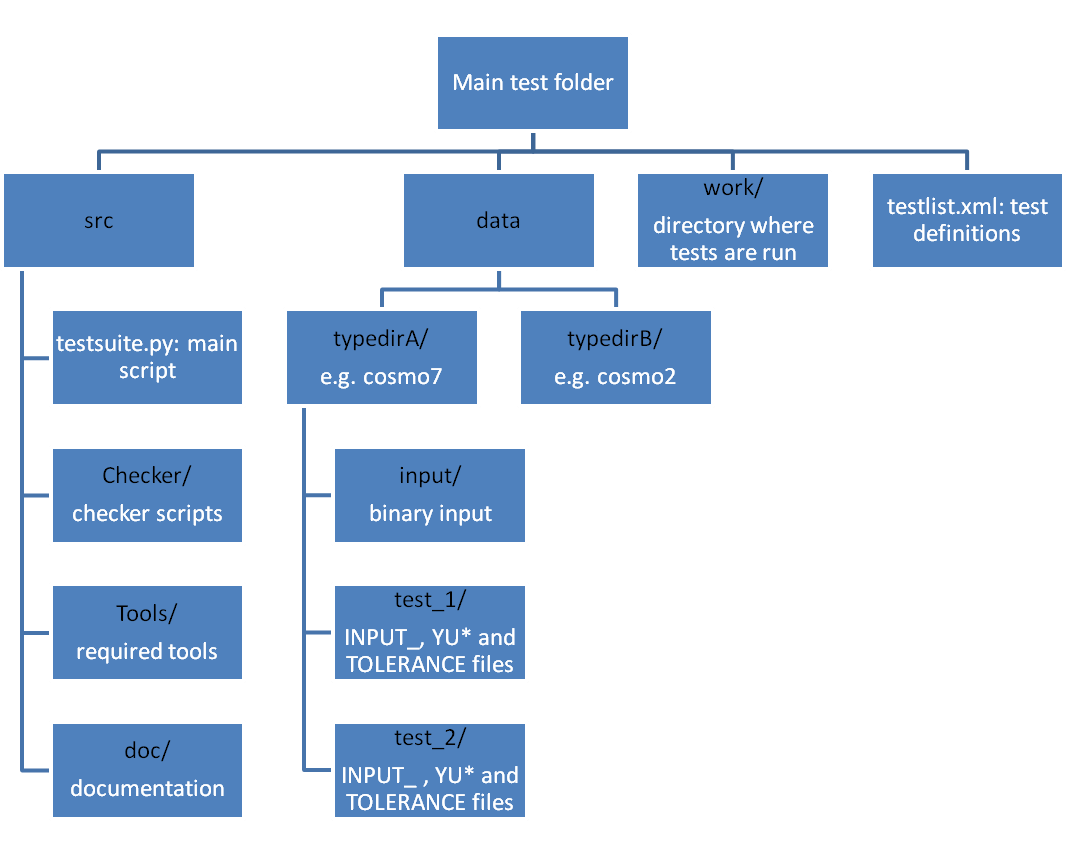
\includegraphics[width=0.7\linewidth]{fig_structure}%
\caption{Test folder organization \label{fig:structure}}
\end{center}
\end{figure}

When running the testsuite, for each of the tests defined in the \texttt{testlist.xml} input file, a separate directory \texttt{work/}type\texttt{/}testname\texttt{/} is created. First, the executable, namelists and auxiliary files are copied and the binary input linked into this folder. Then, the test simulation is run in this working directory. The working directories for the tests are not deleted after execution; if a test failed the user can thus go return manually to these directories for further investigation.

%---------------------------------------------------------------------
\newpage
\section{Command line arguments}

Command line arguments are used to control the execution of the main \texttt{testsuite.py} script. Below is a complete list of available arguments, where the default values/options are given in square brackets:\\

\begin{longtable}{lp{10cm}}
\texttt{-h}, \texttt{--help} & Print the help message.\\[1.2ex]
\texttt{-n} NPROCS & Number of processors (nprocx*nprocy+nprocio) to use [16].\\[1.2ex]
\texttt{--nprocio=}NPROCIO & Set number of aynchronous IO processor [as specified in namelist]. If this argument is present it will override any values given in the namelist or \texttt{testlist.xml} file.\\[1.2ex]
\texttt{-f}, \texttt{--force} & Do not stop upon error or fail [stop on error].\\[1.2ex]
\texttt{-v} V\_LEVEL & Verbosity level from 0 (quiet) to 3 (very verbose) [1].\\[1.2ex]
\texttt{--mpicmd=}MPICMD & MPI run command (e.g. "mpirun -n") ["aprun -n"].\\[1.2ex]
\texttt{--exe=}EXE & Executable file, [as specified in \texttt{testlist.xml}]. If this argument is present it will override any values given in the \texttt{testlist.xml}.\\[1.2ex]
\texttt{--color} & Select colored output.\\[1.2ex]
\texttt{--steps=}STEPS & Run only specified number of timesteps. If this argument is present it will override any values given in the \texttt{testlist.xml}.\\[1.2ex]
\texttt{-w}, \texttt{--wrapper} & Use wrapper instead of executable for mpicmd (useful for OpenMPI on Mac computers).\\[1.2ex]
\texttt{-o} STDOUT & Redirect standard output to selected file.\\[1.2ex]
\texttt{-a}, \texttt{--append} & Appends standard output if redirection selected.\\[1.2ex]
\texttt{--only=}ONLY & Select one tests to run (e.g. \texttt{--only=}cosmo7,test\_1).\\[1.2ex]
\texttt{--update-namelist} & Use testsuite to update namelists. The tests will not be executed with this option.\\[1.2ex]
\texttt{--force-match} & Force bit-reproducible results\\[1.2ex]
\texttt{--update-yufiles} & Define new references by copying test output into the test reference folder. The tests will not be executed with this option.\\[1.2ex] 
\texttt{-l} TESTLIST, & Select the xml testlist file [\texttt{testlist.xml}].\\
\texttt{--testlist=}TESTLIST & \\[1.2ex]
\texttt{--workdir=}WORKDIR & Name of working directory \\[1.2ex]
\texttt{--tune-thresholds} & Enable automatic tuning of thresholds files \\[1.2ex]
\texttt{--tuning-iterations=}ITER & Set the number of times tests should be executed. [\texttt{10}]\\[1.2ex]
\texttt{--update-thresholds} & Update the thresholds based on the results of the current run. \\[1.2ex]
\texttt{--reset-thresholds} & Sets all values in threshold files to 0.0 on the first run of a test\\[1.2ex]
\texttt{-t} TIMEOUT & Timeout in s for each test\\[1.2ex]
\texttt{--tolerance=}TOLERANCE & Select the tolerance file name\\[1.2ex]
\end{longtable}

\section{Testsuite configuration}
If a configuration file testsuite\_config.cfg is present in the current
directory it will be read, otherwise the default configuration file in the
testsuite source directory will be used. It contains the following
information:
\begin{verbatim}
# List of INPUT namelist 
# Should be a python list format
l_files = ['INPUT_ORG','INPUT_ASS','INPUT_DIA','INPUT_DYN','INPUT_INI',\
           'INPUT_IO','INPUT_PHY','INPUT_SAT','INPUT_POL','INPUT_IDEAL']
# File containing the parallelisation option (nproc ...)
par_file = INPUT_ORG
# File containing time step information
dt_file = INPUT_ORG
# File containing test result
res_file = TEST_RES
# File used for the tolerance checker
yufile = YUPRTEST
# List of dual parameters (which may be interchanged in the namelists)
# Should be a python list format
dual_params=[('nstop','hstop'),('hincrad','nincrad')]
# Where is the namelist switch for the testsuite output
nl_ts_switch = INPUT_DIA
# Where are all the namelists after execution
config_nl = YUSPECIF
# Is a perturbation necessary
pert_avail = True
\end{verbatim}

%---------------------------------------------------------------------
\newpage
\section{Test specification (\texttt{testlist.xml})}
\label{sec:testlist}
The tests are defined in an XML file named \texttt{testlist.xml} which should be present in the testsuite root directory. It typically is of the following structure:

\begin{verbatim}
<?xml version="1.0" encoding="utf-8"?>
<testlist>

  <!-- ******* COSMO 7 ******* -->

  <test name="test_1" type="cosmo7">
    <description>Only dynamics</description>
    <checker>run_success_check</checker>
    <checker>tolerance_check</checker>
    <changepar file="INPUT_ORG" name="hstop">1</changepar>
    <autoparallel>1</autoparallel>
  </test>
  
  <test name="test_2" type="cosmo7">
    <description>Dynamics and physics</description>
    <namelistdir>cosmo7/test_1</namelistdir>
    <refoutdir>cosmo7/test_2</refoutdir>
    <checker>run_success_check</checker>
    <checker>tolerance_check</checker>
    <changepar file="INPUT_ORG" name="hstop">1</changepar>
    <changepar file="INPUT_ORG" name="lphys">.TRUE.</changepar>
    <autoparallel>1</autoparallel>
  </test>
  
 <\testlist>
\end{verbatim}

The test list is embedded within a \tl \tbf{testlist}\tg \hs tag. Each test is defined by a \tl \tbf{test}\tg  \hs tag, which has two compulsory attributes \tit{name} and \tit{type}. In the above example two tests are defined. The first test (\texttt{test\_1}) will run with namelists and reference data from the \texttt{data/cosmo7/test\_1} directory. Since the directory containing the namelists and reference data are named like the test, they do not need to be further specified. Two checkers will be run, one assuring that the simulation has run correctly and did not crash and one which will check that the results are within thresholds. The namelist parameter \texttt{hstop} is changed to stop the simulation after one hour. Test two uses the same namelists as test one but has its own reference files, thus the directories are specifically given with the optional \texttt{namelistdir} and \texttt{refoutdir} tags. Additionally, the namelist switch \texttt{lphys} is activated, in order to run with physics.

Below a list of the valid XML tags for defining a given test is given. Tags and/or attributes which are optional and need not mandatorily be specified for each test are indicated with an asterixs (*).\\

\begin{tabular}{lp{12cm}}
\texttt{\tl description\tg} & A short description of the test which will be printed out by the testsuite.\\[1.2ex]
\texttt{\tl namelistdir*\tg} & Directory where to find the namelist (\texttt{INPUT\_}*) files for this test. Defaults to \texttt{data/}type\texttt{/}name, where type and name correspond to the type and name of the test, respectively.\\[1.2ex]
\texttt{\tl refoutdir*\tg} & Directory which contains the reference output files (\texttt{YU*}). Defaults to the directory which contains the namelist (see above). If the path starts with ''../'', it will be relative to the running directory, i.e. ''../test\_3'' is equivalent to ''work/typedir/test\_3''. This can be use to compare against another test which has already run.\\[1.2ex]
\texttt{\tl depend*\tg} & Path to test directory on which this test depends. If the path starts with ``../'', it will be relative to the running directory.\\[1.2ex]
\texttt{\tl checker\tg} & Name of the checker to be called with this test. This tag can appear several times to apply more than one checker.\\[1.2ex]
\texttt{\tl executable*\tg} & Define the name of the executable. This tag is only considered if no executable name was given as a command line argument.\\[1.2ex]
\multicolumn{2}{l}{\texttt{\tl changepar* file=}\tit{file}\texttt{ name=}\tit{name}\texttt{ occurence*=}\tit{occurence}\texttt{\tg}}\\
 & Modify the parameter \tit{name} in the namelist \tit{file} to a new value for the current test. The optional \tit{occurence}  attribute can be used to modify a specific occurrence of the parameter in the namelist.\\[1.2ex]
\texttt{\tl autoparallel*\tg} & Number to select a domain decomposition (\texttt{nprocx} x \texttt{nprocy}) within a automatically generated list of decomposition possibilities. Running two tests with different autoparallel numbers will enable to compare runs with different processor configurations.\\[1.2ex]
\end{tabular}


%---------------------------------------------------------------------
\newpage
\section{Checker scripts}
\label{sec:checker}

A checker is an external script which is called from the main testsuite program to verify the correctness of a specific test. More than one checker can be applied to an individual test. For example, the user might want to check whether the run was successful, whether output was produced and whether results are within specified thresholds. The checkers can be written in any scripting language (bash, python ...). Communication of runtime variables between the testsuite and a checker is achieved via environment variables. A checker can access a set of environment variables defined by the testsuite.\\


\begin{tabular}{lp{10cm}}
\texttt{TS\_BASEDIR} & Root directory of the testsuite.\\[1.2ex]
\texttt{TS\_VERBOSE} & Verbosity level requested by the user for running the testsuite.\\[1.2ex]
\texttt{TS\_RUNDIR} & Directory where the current test was run.\\[1.2ex]
\texttt{TS\_LOGFILE} & File which contains the standard output and standard error of the current test.\\[1.2ex]
\texttt{TS\_NAMELISTDIR} & Directory containing the namelist of the current test.\\[1.2ex]
\texttt{TS\_NL\_TS\_SWITCH} & Where the namelist switch for the testsuite output is.\\[1.2ex]
\texttt{TS\_CONFIG\_NL} & Where all the namelists are after execution.\\[1.2ex]
\texttt{TS\_DT\_FILE} & Namelist file containing time step information.\\[1.2ex]
\texttt{TS\_PERT\_AVAIL} & Is a perturbation necessary.\\[1.2ex]
\texttt{TS\_REFOUTDIR} & Directory containing the reference files for the current test.\\[1.2ex]
\texttt{TS\_TUNE\_THRESHOLDS} & Shows whether or not tuning was activated\\[1.2ex]
\texttt{TS\_TUNING\_ITERATIONS} & Number of times each test will be executed if tuning of tolerance files is activated.\\[1.2ex]
\texttt{TS\_RESET\_THRESHOLDS} & Shows if the user activated the reset threshold function.\\[1.2ex]
\end{tabular}

Each checker should return an exit code with the following definition:\\

\begin{tabular}{rlp{10cm}}
0 & {\color{green} MATCH} & Results match bit-by-bit as compared to the reference.\\[1.2ex]
10 & {\color{green} OK} & Results match the reference within defined thresholds.\\[1.2ex]
15 & {\color{grey} SKIP} & Test not applicable and thus skipped.\\[1.2ex]
20 & {\color{red} FAIL} & Test failed, results are outside of thresholds.\\[1.2ex]
30 & {\color{red} CRASH} & Test failed due to model crash.\\[1.2ex]
\end{tabular}

The checkers to be called for a given test are defined within the \texttt{testlist.xml} file. All checkers are called irrespective of the exit code of preceding tests. The overall status of a test is defined as the maximum of the exit codes of all checkers called.

\subsection{The run success checker}

The \texttt{run\_success\_check.py} checker will check the successful execution of the test. It searches the standard output of the simulation for the typical \texttt{CLEAN UP} message issued at the end of a successful model simulation.

\subsection{The grib output checker}

The \texttt{existence\_grib\_out.sh} checker will check whether a simulation has correctly written at least one GRIB output file (e.g. \texttt{lfff00000000}) and that this file is of non-zero size.

\subsection{The identical checker}

When bit identical results are expected, as for example when comparing two different parallelizations on a given system, the \texttt{identical\_check.py} checker should be called. This checker expects a \texttt{YUPRTEST} output file (see below) and absolute differences between the output of the test and the reference file are compared to within a zero tolerance threshold.\\
Note that bit identical results can only be expected when two simulations are run on the same system. A test using the \texttt{identical\_check.py} should always have reference directory pointing to a previous test in the working folder, e.g. \texttt{\tl refoutdir\tg../test\_3\tl refoutdir\tg}.

\subsection{The tolerance checker}

In order to validate COSMO results a specific output file named \texttt{YUPRTEST} output file is used. This file, which contains double precision values of the min, max and mean of the prognostic variables on each model level at specific time steps, is written out when the parameter \texttt{ltestsuite=.TRUE.} is activated in the \texttt{DIACTL} namelist group in the \texttt{INPUT\_DIA} namelist file.\\
When compiling the code on a different architecture, or when introducing some technical modification (e.g. optimization), one does not expect bit identical results with respect to the previous model version. The \texttt{tolerance\_check.py} script will compare results to a reference but accounting for rounding errors and allowing to compare output files within some tolerance values.\\
The definition of meaningful thresholds is not a straightforward task as they should be low enough to detect bugs in the software, while allowing to tolerate acceptable rounding error differences. So far the following approach was adopted to determine these thresholds:
\begin{itemize}
	\item two COSMO executable are generated with two different compilers
	\item at each time step a perturbation is added to the prognostic variables
	\begin{equation}
	    f=f\,(1+R\,\epsilon) \; \; \mbox{with} \; \; \epsilon=1^{-15} \; \; \mbox{and} \; \; R  \; \; \mbox{random a perturbation}
	\end{equation} 
\end{itemize}

The maximum errors obtained for different time steps by running and comparing these two executables N times (typically N=30) are used as threshold values.\\

\subsection{Creation of Tolerance Files}

The tolerance checker is able to tune these files automatically. 
The tuning process starts the same way a normal run of the tolerance checker would, with the comparison of the two \texttt{YUPRTEST} files. The compare phase is followed by the tuning of failed comparisons this is accomplished by increasing the corresponding levels threshold with a predefined factor. The checker always returns {\color{green} OK} during the tuning process.
The argument \texttt{--tune-thresholds} will enable automatic tuning mode which will tune the tolerance files. \\ 
The process of tuning can be furthermore configured by using the following arguments:

\begin{itemize}
    \item \texttt{--tuning-iterations=N} - Specifies the number of tuning iterations. The default is 10.
	\item \texttt{--reset-thresholds} - The tolerance files corresponding to the current test will be reset on the first run. So that each value is set to 0.0 which results in a tuning from scratch.
	\item \texttt{--update-thresholds} - Update the thresholds based on the results of the current run.
\end{itemize}

\subsection{Custom checkers}

Users are encouraged to develop, document and share their own checker scripts which can be compiled and distributed with future versions of the testsuite.

\section{Updating or generating reference files}

When a new version of COSMO with significant changes is released, for instance with a new physics scheme or with new tuning parameter values, the reference files (e.g. \texttt{YUPRTEST}) need to be updated. To this end, the \texttt{testsuite.py} script can be called with the \texttt{--update\_yufiles} option, which will copy the reference files from the test directories back into the reference directories. Care should be taken that this is only done under the following conditions:
\begin{itemize}
    \item The user is sure that all tests run successfully and the eventual failing tests are due to model changes (which have been thoroughly checked and tested).
    \item The testsuite has been previously run fully (using the \texttt{--force} option) and without specifying only a limited number of tests (e.g. \texttt{--skip=} or \texttt{--only=}) or a limited number of timesteps (e.g. \texttt{--steps=}).
\end{itemize}

\end{document}
